\section{}
\[
H(s)=\frac{10\sqrt{202}\,s}{(s+1)(s+10)}\,.
\]
\subsection{Bode-Diagramm}
\begin{center}
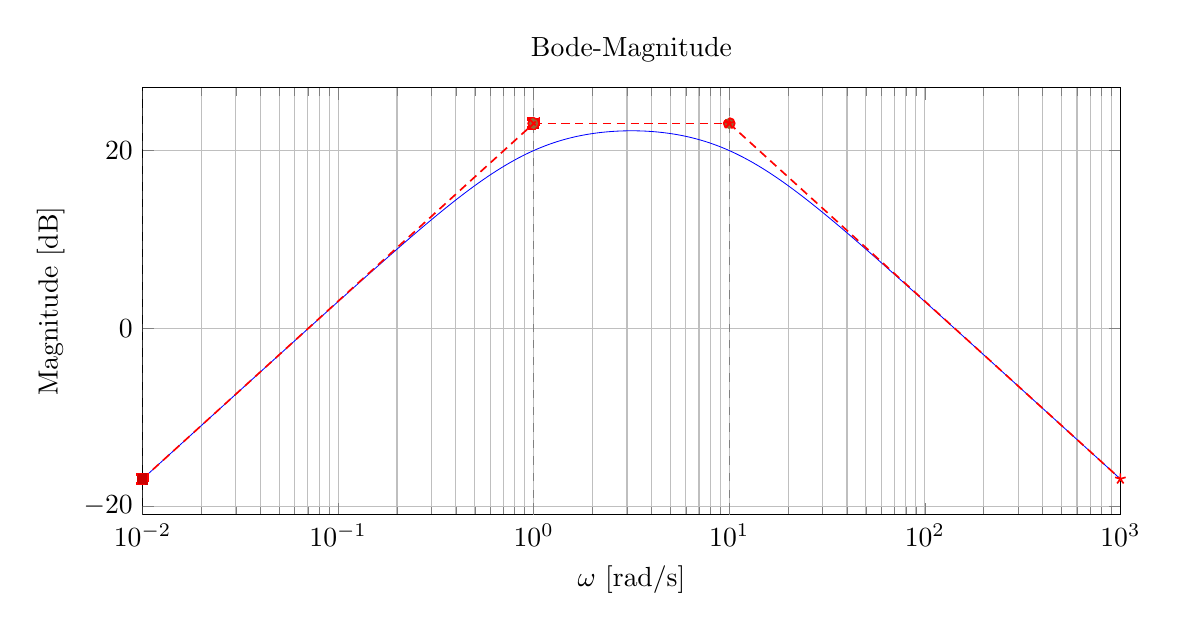
\begin{tikzpicture}
\begin{semilogxaxis}[
  width=14cm,height=7cm,
  xmin=1e-2,xmax=1e3,
  xlabel={$\omega$ [rad/s]},
  ylabel={Magnitude [dB]},
  ytick distance=20,
  grid=both,
  title={Bode-Magnitude}
]
\addplot[
  domain=1e-2:1e3,
  samples=600,
  mark=none,
  line width=0.3pt,
  blue
] {20 + 10*ln(202)/ln(10) + 20*ln(x)/ln(10) - 20*ln(sqrt(1 + x^2))/ln(10) - 20*ln(sqrt(100 + x^2))/ln(10)};
\addplot+[domain=1e-2:1,samples=2,dashed,dash pattern=on 3pt off 2pt,line width=0.6pt,red] {10*ln(202)/ln(10) + 20*ln(x)/ln(10)};
\addplot+[domain=1:1e1,samples=2,dashed,dash pattern=on 3pt off 2pt,line width=0.6pt,red] {10*ln(202)/ln(10)};
\addplot+[domain=1e1:1e3,samples=2,dashed,dash pattern=on 3pt off 2pt,line width=0.6pt,red] {10*ln(202)/ln(10) - 20*ln(x/10)/ln(10)};
\draw[gray,dashed] (rel axis cs:0,0) -- (rel axis cs:0,1);
\draw[gray,dashed] (axis cs:1,\pgfkeysvalueof{/pgfplots/ymin}) -- (axis cs:1,\pgfkeysvalueof{/pgfplots/ymax});
\draw[gray,dashed] (axis cs:10,\pgfkeysvalueof{/pgfplots/ymin}) -- (axis cs:10,\pgfkeysvalueof{/pgfplots/ymax});
\node[gray,anchor=south east] at (axis cs:1,\pgfkeysvalueof{/pgfplots/ymax}) {\scriptsize Pol $\omega_{p1}=1$};
\node[gray,anchor=south east] at (axis cs:10,\pgfkeysvalueof{/pgfplots/ymax}) {\scriptsize Pol $\omega_{p2}=10$};
\end{semilogxaxis}
\end{tikzpicture}
\vspace{6mm}
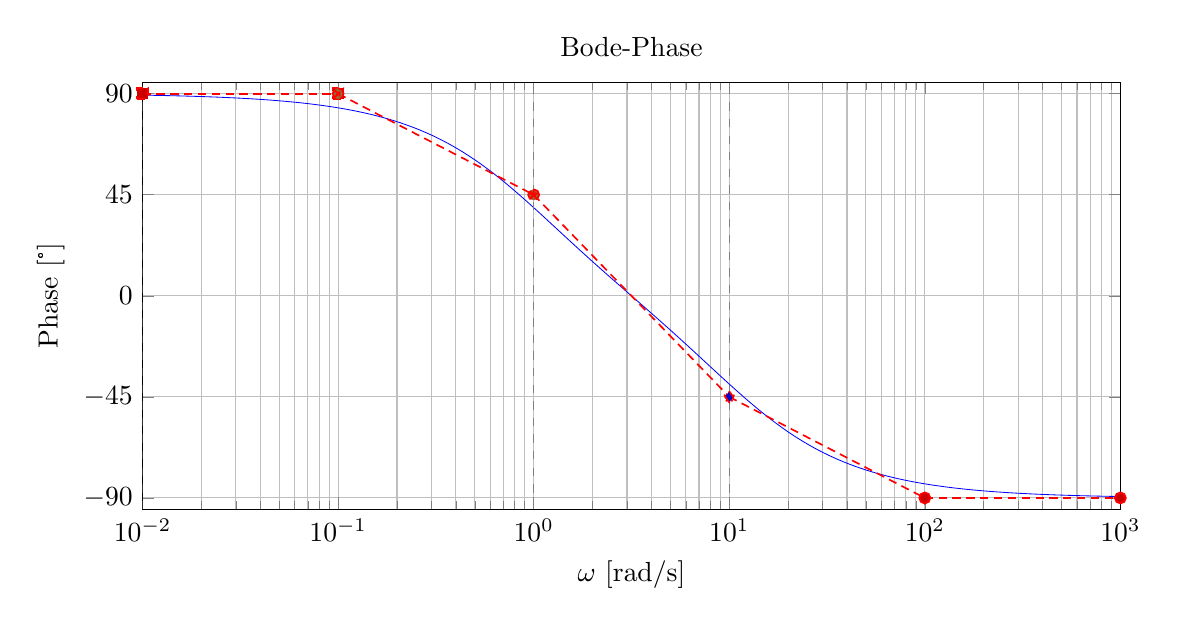
\begin{tikzpicture}
\begin{semilogxaxis}[
  width=14cm,height=7cm,
  xmin=1e-2,xmax=1e3,
  ymin=-95,ymax=95,
  ytick distance=45,
  xlabel={$\omega$ [rad/s]},
  ylabel={Phase [°]},
  grid=both,
  title={Bode-Phase}
]
\addplot[
  domain=1e-2:1e3,
  samples=600,
  mark=none,
  line width=0.3pt,
  blue
] {90 - atan(x) - atan(x/10)};
\addplot+[domain=1e-2:1e-1,samples=2,dashed,dash pattern=on 3pt off 2pt,line width=0.6pt,red] {90};
\addplot+[domain=1e-1:1e0,samples=2,dashed,dash pattern=on 3pt off 2pt,line width=0.6pt,red] {45 - 45*ln(x)/ln(10)};
\addplot+[domain=1e0:1e1,samples=2,dashed,dash pattern=on 3pt off 2pt,line width=0.6pt,red]{45 - 90*ln(x)/ln(10)};
\addplot+[domain=1e1:1e2,samples=2,dashed,dash pattern=on 3pt off 2pt,line width=0.6pt,red]{-45 - 45*ln(x/10)/ln(10)}; % bei 10: -45°, bei 100: -90°

\addplot+[domain=1e2:1e3,samples=2,dashed,dash pattern=on 3pt off 2pt,line width=0.6pt,red] {-90};
\draw[gray,dashed] (rel axis cs:0,0) -- (rel axis cs:0,1);
\draw[gray,dashed] (axis cs:1,\pgfkeysvalueof{/pgfplots/ymin}) -- (axis cs:1,\pgfkeysvalueof{/pgfplots/ymax});
\draw[gray,dashed] (axis cs:10,\pgfkeysvalueof{/pgfplots/ymin}) -- (axis cs:10,\pgfkeysvalueof{/pgfplots/ymax});
\node[gray,anchor=south east] at (axis cs:1,\pgfkeysvalueof{/pgfplots/ymax}) {\scriptsize Pol $\omega_{p1}=1$};
\node[gray,anchor=south east] at (axis cs:10,\pgfkeysvalueof{/pgfplots/ymax}) {\scriptsize Pol $\omega_{p2}=10$};
\end{semilogxaxis}
\end{tikzpicture}
\end{center}
\newpage
\subsection{Erklärung}
\vspace{5mm}
\begin{description}[leftmargin=1.2em,labelsep=.6em,font=\bfseries]
\item[Schritt 1] Nullstelle im Ursprung: $H(s)=10\sqrt{202}\,\dfrac{s}{(s+1)(s+10)}$. Für $\omega\ll1$ gilt $|H(\j\omega)|\approx \sqrt{202}\,\omega$; Startsteigung $+20\,\mathrm{dB/dec}$ mit Startniveau $10\log_{10}202\,\mathrm{dB}$. Startphase $\approx+90^\circ$.
\item[Schritt 2] Pol bei $\omega_{p1}=1\,\mathrm{rad/s}$: ab $\omega=1$ Steigungswechsel um $-20\,\mathrm{dB/dec}$; Zwischenbereich $[1,10]$ ist betragsflach. Exakt $|H(\j1)|=\dfrac{10\sqrt{202}}{\sqrt{2}\sqrt{101}}=10\Rightarrow20\,\mathrm{dB}$ (symmetrische Ecklage). Phasenabfall um $90^\circ$ über $\omega\in[0.1,10]$; Geradennäherung $45^\circ-45^\circ\log_{10}\omega$.
\item[Schritt 3] Pol bei $\omega_{p2}=10\,\mathrm{rad/s}$: ab $\omega=10$ weiterer Steigungswechsel um $-20\,\mathrm{dB/dec}$; Gesamtslope $\,-20\,\mathrm{dB/dec}$ für $\omega\gg10$. Auch hier $|H(\j10)|=\dfrac{100\sqrt{202}}{\sqrt{101}\sqrt{200}}=10\Rightarrow20\,\mathrm{dB}$. Der zweite Pol senkt die Phase um weitere $90^\circ$ in $\omega\in[1,100]$; Geradennäherung $-45^\circ\log_{10}(\omega/10)$, Grenzwert $\angle H\to-90^\circ$.
\end{description}

\vspace{0.5cm}
\medskip
\noindent\textbf{Stückweise Näherung}
\[
|H(\j\omega)|_{\mathrm{dB}}\approx
\begin{cases}
10\log_{10}202+20\log_{10}\omega,& \omega\ll1,\\[4pt]
20,& \omega=1,\\[4pt]
10\log_{10}202,& 1\ll\omega\ll10,\\[4pt]
20,& \omega=10,\\[4pt]
10\log_{10}202-20\log_{10}(\omega/10),& \omega\gg10,
\end{cases}
\qquad
\]
\newpage